\chapter{Europium Experiments}\label{ch:eu_exp}

Previous experiments have been able to detect small quantities of liquid
europium using absorption spectroscopy in the ultraviolet \cite{Yun:2001wc}.
However, the most interesting transitions for europium occur in the visible due
to the high efficiencies of the fluorescence decay pathway in europium. Under
these conditions, it is difficult to acquire an accurate absorption spectrum
for analysis of concentration or natural radiative lifetimes. To date, it
appears that within the visible the lowest concentration ever measured is
200\,mM of aqueous europium. This has been measured using complex
spectrophotometers and through \ac{PAS} \cite{Sawada:1979vca}.

These experimental results reveal a few interesting factors about
europium's electronic transitions (see Figure~\ref{fig:eu_spec_theory}.
First, the forbidden transitions are not much weaker than the allowed
$^7F_0 \leftrightarrow ^5D_2$ transition near 464nm, which occurs when
nonlinear effects to the electronic wave functions play a dominant role
\cite{Walsh:2005te}. A second unexpected attribute was noted in the forbidden
$^7F_0 \leftrightarrow ^5D_0$ transition indicating that this absorption
peak was incredibly small in comparison to other transitions in the aqueous
europium spectrum \cite{Sawada:1979vca}. The authors who noted this
peculiarity suggests that the thinness is due to hypersensitivity of the
transition to the environment that the europium is in, leading to a squeezing
effect of the spectral line that overpowers the broadening effects.

It is important, especially for the applications discussed in
section~\ref{subsec:eu_beads}, to be able to detect aqueous europium at
much smaller concentrations than 200\,mM in the visible. As the proceeding
discussion shows, \ac{BBCEAS} is uniquely apt at being able to determine
minute quantities of aqueous europium in a way that provides qualitative
data about the fluorescence transitions that is most possible through other
methods. As such, the experimental setup designed in chapter~\ref{ch:bbceas}
was used to determine just how low of a limit of detection could be obtained
with \ac{BBCEAS}.



\section{Measurements using BBCEAS}\label{sec:eu_measurements}

\begin{figure}[t]
\begin{center}
\includegraphics[]{figures/plots/eu_conc/eu_conc.pdf}
\end{center}
\caption[Europium Absorption Spectra at different Concentrations]{Europium absorption spectrum taken at different concentrations, with w reference from Sawada 1979 \cite{Sawada:1979vca}. The peaks are noticeable even though the spectra appear different. The peculiar undulations between expected peaks are due to laser fluctuations. The shaded areas represent one standard deviation of error. The larger error near 600\,nm is due to low light intensity in that range after the 585\,nm edgepass filter.}
\label{fig:eu_conc}
\end{figure}

With experimental and theoretical results indicating what should be seen in
an absorption spectrum, the \ac{BBCEAS} technique was applied to measure
small concentrations of liquid europium in the visible, at concentrations
lower than the 200\,mM seen in the literature \cite{Sawada:1979vca}. This
was accomplished using the same technique used to perform the rhodamine 6G
calibrations in chapter \ref{ch:cal}.

As one can see from figure~\ref{fig:eu_conc}, the major electronic transitions
were easily observed. However, as one can see from the figure, it is difficult
to determine why the measured spectrum has a higher baseline, and why the
relative intensities between the transitions do not match those in the
literature. Since altering of the intensity of the a transition can occur
when a substance is optically saturated, the experiment was repeated at lower
powers.

\begin{figure}[t]
\begin{center}
  \includegraphics[]{figures/plots/eu_power/eu_power.pdf}
\end{center}
\caption[Europium Absorption Spectra at different Input Intensities]{Europium absorption spectrum taken at different powers. These spectra are cleaner than in Figure~\ref{fig:eu_conc} due to better control over the laser fluctuations. The similar shapes between input powers indicates that optical saturation was not a factor in causing the undulations in Figure~\ref{fig:eu_conc}.}
\label{fig:eu_power}
\end{figure}

Figure~\ref{fig:eu_power} debunks the idea of optical saturation because the
absorption spectra are similar at many different input powers to the cavity,
even though the highest power in the set of the experiments is the same as
the original. This peculiar result is likely due to laser fluctuations in
the original liquid europium measurements. The intensity fluctuations would
increase the intensity of the peaks relative to each other and cause some line
broadening because the the laser fluctuation is a function of time \emph{and}
wavelength: see section~\ref{subsec:laser_fluc}.

Measurements were also performed on a variety of concentrations. This resulted
in a minimal detection limit of approximately 5\,mM in the visible, a 40 fold
improvement in the limit of detection against what is commonly seen in the
literature. This sensitivity is based on equation \eqref{eq:ceas_err_geo}.

These results indicate that \ac{BBCEAS} can be used to detect liquid Eu(III)
at a lower concentration than what was possible before. With modifications to
the \ac{BBCEAS} setup discussed in section~\ref{sec:bbceas_enhance} it will be
possible to lower the detectable concentration to the micromolar range because
the major source of experimental error -- the intensity fluctuations -- will be eliminated.



\section{Further Investigations of Europium}\label{sec:eu_future}

In this chapter it has been shown that preliminary \ac{BBCEAS} testing of
Eu(III) in aqueous solution can be detected in much smaller quantities than
previously reported in the literature.  This detection limit, combined with
coordination complexes, can be used to better understand europium complexes and
to illuminate how to use such complexes effectively.



\subsection{Europium Complexes}\label{subsec:eu_complex}


\begin{wrapfigure}{o}{\marginspace}
\begin{center}
  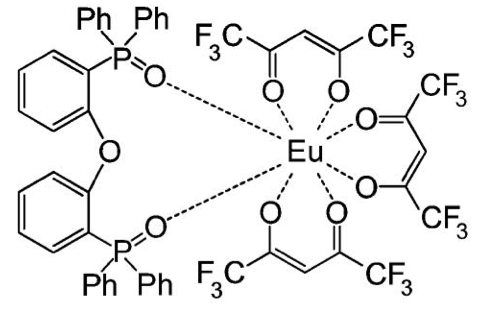
\includegraphics[width=\marginspace]{figures/eu_complex.png}
\end{center}
\emph{\footnotesize{\raggedright{A europium complex \cite{Wilson:2010hs}}}}
\end{wrapfigure}

It is quite tricky to measure the absorption spectrum of europium
and detect any fluorescence due to the extremely low absorption
cross sections of the europium ion. Coordination complexes
alleviate this problem by acting as ``catcher's mitts'', which
dramatically increase the probability of a photon being absorbed
\cite{Kirby:1983cl,Sveshnikova:2000cr,Werts:2002fs,Bunzli:2005ic,Moudam:2009in,Wilson:2010hs,Harma:2010dm,InstituteofBiomedicine:2011vt,Pihlasalo:2012cq}.
Combined with the high fluorescence quantum efficiency of the europium
complexes, these coordination systems increase the usability of europium by
allowing even moderate intensity light sources to induce fluorescence of high
spectral purity.

However, to calculate the theoretical parameters for such a system, it is
necessary to measure the time required for an excited europium complex to decay
down to the ground state. As shown from equations \eqref{eq:nat_life_emiss},
\eqref{eq:nat_life_abs} and \eqref{eq:branch_ratio}, it is possible to use the
absorption and emission spectrum of a given transition to determine the natural
radiative lifetime of the complex, transition probabilities and branching
ratios. This information is necessary to acquire a better theoretical
understanding of the electron configuration and interaction in europium
complexes. The derived theory can then be used to optimise coordination
complexes to acquire the highest fluorescence yields, or more spectrally pure
fluorescence by the reduction or enhancement of certain electron dipole
transitions. This information could be useful to engineers attempting to design
\acp{OLED}, as they could engineer the intensity and spectral bands at which
the complexes would fluoresce.



\subsection{Europium Complexes adsorbed to Polystyrene Beads}\label{subsec:eu_beads}

\begin{figure}[t]
\begin{center}
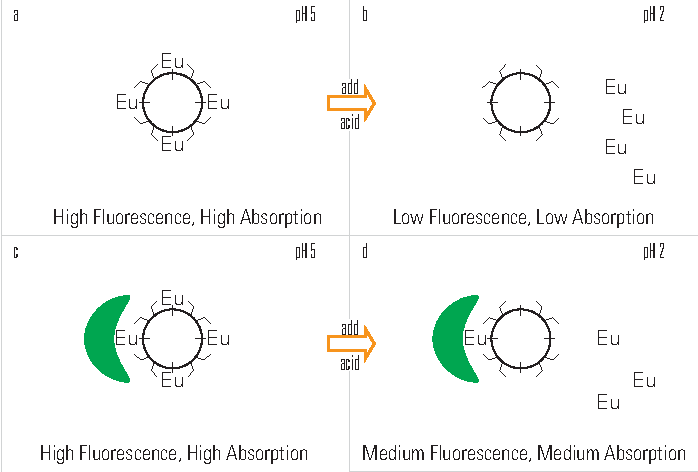
\includegraphics[]{figures/eu_beads/eu_beads.pdf}
\end{center}
\caption[Europium Bead Protein Assay]{When polystyrene beads coated with europium complexes (a) are exposed to an acidic environment (b), the complexes dissolve, reducing the absorption and fluorescence signal given off by europium. If, however, a biomolecule is adhered to the surface (through ionic interactions, c), then the europium under the molecule is prevented from leaving its complex (d). This keeps the absorption and fluorescence signals high, and how high these signals are can be used to determine both the quantity of biomolecules in a solution on a molecule by molecule basis.}
\label{fig:eu_beads}
\end{figure}

Europium complexes have been used as fluorescent markers and for displays,
among other applications. However, a recent paper provides an interesting use
of europium complexes attached to nano polystyrene beads. These beads are able
to hold tens of thousands of chelated europium complexes on one bead. While
this is interesting on its own as a way to produce highly localised intense
fluorescence, the beads also have an additional property that makes them useful
for detections of larger biomolecules and cells: the beads are designed with a
negative surface potential, even with the europium complexes attached.

This is useful because many proteins and cells will adhere to the surface of
the beads. If a europium ion attempts to disassociate from its coordination
complex, it is sterically hindered from doing so. In highly acidic solutions --
around a pH of 2 -- europium tends to disassociate from its complex readily,
which reduces the fluorescence signal. However, since attached biomolecules
prevent this dissociation through steric hindrance, it is possible to use the
ratio of the observed fluorescence in a biomolecule solution to the background
fluorescence upon all the complexes dissociating to calculate the amount of a
biomolecule there is in a solution.

Detecting the concentration of a biomolecule is currently done using
fluorescence properties of europium complexes. However, absorption techniques
can lead to higher sensitivities and lower limits of detection because the
absorption measurement does not need to account for a large scattering
angle, unlike fluorescence where an emitted photon could travel in any
direction.\marginpar{This is to say it is easier to detect the reduction of
photons due to absorption than it is to pray that an emitted photon will
travel in the correct direction.} As such, a \ac{BBCEAS} measurement of the
absorption spectrum of a biomolecule solution laced with europium complexes
should lead to even greater sensitivities and lower limits of detection than
currently stated in the literature.

Additionally, the speed of \ac{BBCEAS} measurements would greatly decrease the
time required to acquire biomolecule concentrations to only a few minutes.
Besides the clear advantage of fast molecular concentration determination, the
fast acquisition of the absorption spectrum allows for detection limits that
are lower than the fluorescence measurements by measuring the \emph{rate
constant} for the decay process. In this manner, even concentrations of
biomolecules that did not create a significant shift from no biomolecule
samples could still be determined using the slow down of the decay of the
absorption signal versus a blank sample.

Extra benefits can be found from the property that the electronic dipole
transitions in europium complexes will alter due to the adsorption of a
biomolecule onto the bead. Judd-Ofelt theory allows for many of the forbidden
transitions provided a higher order interaction with a localised electric
field, which can come from a complex or the surrounding medium. As such,
parameters such as the branching ratio and natural radiative lifetime would be
affected by the biomolecule attached to the europium bead. This would prove to
be a novel approach to not only detecting minuscule concentrations of proteins
in a solution, but would also allow for the adsorbed protein on the beads to
be identified. It is feasible to believe that this identification process
could be done to multiple biomolecules simultaneously, creating a single
molecular probe for determining the concentrations of different proteins in a
molecular soup, such as a cell lysate sample.

With the ability to achieve lower limits of detection, higher sensitivities,
fast acquisition and biomolecule identification, \ac{BBCEAS} detection of
europium complex beads provides a tantalising alternative to traditional
biomolecule detection techniques. \ac{BBCEAS} could be integrated into
microtiter pipette plates to provide an all in one solution for rapidly
testing concentrations of cell lysates or other samples.



\section*{Chapter Review}

Europium is a complicated metal. It is difficult to detect in a solution,
readily reacts with its neighbors, and is only partially understood from a
theoretical basis. However, the \ac{BBCEAS} technique created in chapter
\ref{ch:bbceas} has proven to be useful in both in lowering the limit of
detection for aqueous europium and in acquiring useful, broad spectra that
can be used to calculate parameters such as the natural radiative lifetime of
a transition. With the work laid out in this chapter, it will be possible to
combine \ac{BBCEAS} with europium complexes to create truly amazing protein
assays that detect not only minuscule quantities of proteins but can also
identify which proteins are in a solution.
